\begin{figure}[ht]
\centering
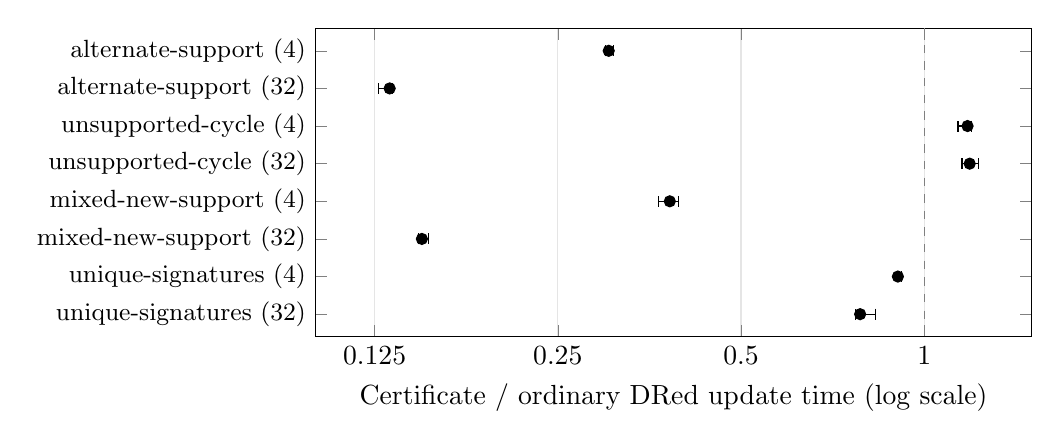
\begin{tikzpicture}
\begin{axis}[width=0.88\linewidth,height=5.5cm,xmode=log,
xmin=0.1,xmax=1.5,ymin=-0.6,ymax=7.6,
ytick={0,1,2,3,4,5,6,7},
yticklabels={alternate-support (4),alternate-support (32),unsupported-cycle (4),unsupported-cycle (32),mixed-new-support (4),mixed-new-support (32),unique-signatures (4),unique-signatures (32)},
yticklabel style={font=\small},y dir=reverse,
xlabel={Certificate / ordinary DRed update time (log scale)},
xtick={0.125,0.25,0.5,1},xticklabels={0.125,0.25,0.5,1},
xmajorgrids=true,grid style={gray!20}]
\addplot[gray,dashed] coordinates {(1,-0.6) (1,7.6)};
\addplot[only marks,mark=*,black,error bars/.cd,x dir=both,x explicit]
coordinates {
(0.303107186,0) += (0.005380192,0) -= (0.003875500,0)
(0.132315292,1) += (0.001499708,0) -= (0.005665689,0)
(1.178358201,2) += (0.016322907,0) -= (0.041958422,0)
(1.187932124,3) += (0.040023678,0) -= (0.034218154,0)
(0.381928514,4) += (0.012880738,0) -= (0.016163149,0)
(0.149473165,5) += (0.003692939,0) -= (0.001777688,0)
(0.905277511,6) += (0.011728574,0) -= (0.005298335,0)
(0.784898536,7) += (0.047034643,0) -= (0.012522867,0)
};
\end{axis}
\end{tikzpicture}
\caption{Post-hoc support replication. Points are median paired ratios; bars are descriptive paired-bootstrap intervals. Values left of one favor certificates; unsupported cycles expose their overhead.}
\label{fig:support}
\end{figure}
